% !TeX spellcheck = en_GB
\documentclass{article}


\usepackage{fancyhdr} % Required for custom headers
\usepackage{lastpage} % Required to determine the last page for the footer
\usepackage{extramarks} % Required for headers and footers
\usepackage[usenames,dvipsnames]{color} % Required for custom colors
\usepackage{graphicx} % Required to insert images
\usepackage{subcaption}
\usepackage{courier} % Required for the courier font
\usepackage{enumerate}
\usepackage{amssymb}
\usepackage{amsmath}
\usepackage{array}
\usepackage{alphalph}
\usepackage{pdflscape}
\usepackage{afterpage}
\usepackage{capt-of}% or use the larger `caption` package
\usepackage{float}
\usepackage{titlesec}
\usepackage{algorithm}
\usepackage[noend]{algpseudocode}

%----------------------------------------------------------------------------------------
% Page setup information

\renewcommand*{\thesubfigure}{%
	\alphalph{\value{subfigure}}%
}%
% !TeX spellcheck = en_GB

% Margins
\topmargin=-0.45in
\evensidemargin=0in
\oddsidemargin=0in
\textwidth=6.5in
\textheight=9.0in
\headsep=0.25in

\linespread{1.1} % Line spacing

% Set up the header and footer
\pagestyle{fancy}
\chead{\compName: \docTitle} % Top center head
\rhead{\firstxmark} % Top right header
\lfoot{\lastxmark} % Bottom left footer
\cfoot{} % Bottom center footer
\rfoot{Page\ \thepage\ of\ \protect\pageref{LastPage}} % Bottom right footer
\renewcommand\headrulewidth{0.4pt} % Size of the header rule
\renewcommand\footrulewidth{0.4pt} % Size of the footer rule

\setlength\parindent{0pt} % Removes all indentation from paragraphs

% Set up section header formatting
\titleformat{\section}{\large \bfseries}{\thesection.}{0.5em}{}
% \titlespacing{\section}{0pt}{15pt}{6pt} % Uncomment to adjust paragraph spacing after section headings

% ----------------------------------------------------------------
% Title stuff
\newcommand{\docTitle}{Embedded Subsystem}
\newcommand{\compName}{CAN-RGX}
\newcommand{\authorName}{Hanzhen Lin, Tyler Gamvrelis, Twesh Upadhyaya}

\title{
	\vspace{2in}
	\textmd{\textbf{\compName:\ \docTitle}}\\
	\vspace{0.1in}
	\vspace{3in}
}

\author{\textbf{\authorName}}

% ----------------------------------------------------------------
\begin{document}
\maketitle
\clearpage

%
%
%
%

\section*{Introduction} \label{intro}
This document describes the embedded subsystem onboard team ``FAM"'s (fluids affect by magnetism) experiment for the Canadian Reduced Gravity Experiment Design Challenge.

\clearpage

%
%
%
%

% ----------------------------------------------------------------
\tableofcontents
\clearpage


%
%
%
%

\section{Overview} \label{overview}
The embedded subsystem is responsible for acquiring data from sensors, using this data to initiate control sequences, and streaming data to the onboard PC. The sensors are as follows:

\begin{enumerate}
	\item MPU9250: 3-axis accelerometer, gyroscope, and magnetometer, 1 in quantity
	\item 18B20: 1-wire digital temperature sensor, 10 in quantity
\end{enumerate}

The systems to which control signals will be asserted are as follows:

\begin{enumerate}
	\item DRV8871: H-bridge, 6 in quantity
	\item TEC: thermoelectric cooler, 2 in quantity
\end{enumerate}

The proceeding sections will describe each of these in more detail, and subsequently, their integration will be described.

\clearpage

%
%
%
%

\section{MPU9250 (accelerometer, gyroscope, magnetometer)} \label{MPU}
As the MPU9250 measures acceleration, it is capable of automatically triggering the experiment through software once the acceleration magnitude is below a certain threshold. It can also detect other events of interest throughout the flight. All these events can be detected according to the following algorithm, where:

\begin{enumerate}
	\item $w_y$ is the rate of change of the pitch of the aircraft about the y-axis (also called \textit{angular rate}). Note that pitch is the angle between the nose of the aircraft and the horizon % I assume degree/s???
	
	\item $a_z$ is the vertical acceleration of the aircraft. \textbf{Note that $a_z > 0$ implies the aircraft is accelerating downward}.
\end{enumerate}

\begin{algorithm}
	\caption{Algorithm for triggering flight events}
	\begin{algorithmic}[1]
		\Procedure{FlightEvents}{}
			\State{Measure $w_y$ and $a_y$}
			\If{$w_y > 2.5$ AND $a_z < -14.715 \ (1.5G)$}
				\State \Return{Transition from Straight and level to Pull Up}
				
			\ElsIf{$w_y < 0$ AND $a_z > -0.981 \ (0.1G)$}
				% If aircraft is changing its pitch to be more downward and is accelerating upward at less than 0.1G...
				\State \Return{Transition from Pull-up to Reduced Gravity}
				
			\ElsIf{$w_y > 0$ AND $a_z < -0.981 \ (0.1G)$}
				% If aircraft is changing its pitch to be more upward and is accelerating upward at more than 0.1G...
				\State \Return{Transition from Reduced Gravity to Pull-Out}
				
			\Else
				\State \Return{No flight event}
				
			\EndIf
		\EndProcedure
	\end{algorithmic}
\end{algorithm}

\textbf{Note:} It was suggested that a manual mechanism be provided to trigger the experiment in addition to the automated software protocol
\newline
\newline

The MPU9250 is also used to measure the magnetic field generated by the electromagnet. This allows the magnetic field to be generated to its maximum possible value while maintaining safety limits.
\newline
\newline
At a minimum, the MPU9250 must be used to measure the following:
\begin{itemize}
	\item $a_z$ (16 bits, full-scale range $\pm 2g$)
	\item $w_y$ (16 bits, full-scale range $\pm 250 \ [\deg/s]$)
	\item $H_x$, $H_y$, $H_z$ (14 bits each, full-scale range $\pm 4912 \ [uT]$)
\end{itemize}

Note that these full-scale ranges were the defaults and also the most suitable since they provided the highest resolution for the window of interest. Note that the full-scale range of 4912 for $H_i$ was taken from page 50 of the register map, while the datasheet specific 4800.
\newline
\newline

Due to the importance of the readings from the MPU9250, it was decided that the motion processing algorithms should be run at a high rate, about 500 [Hz]. Also, note that the MPU9250 features offset registers that can be user-programmed to eliminate dc offsets. It also features an integrated digital low-pass filter whose bandwidth can be set using the \texttt{DLPF\_CFG} and \texttt{A\_DLFPCFG} for the gyroscope and accelerometer, respectively. Note that lower bandwidth comes at the cost of increased delay, on the order of milliseconds.

\begin{figure}
	\centering
	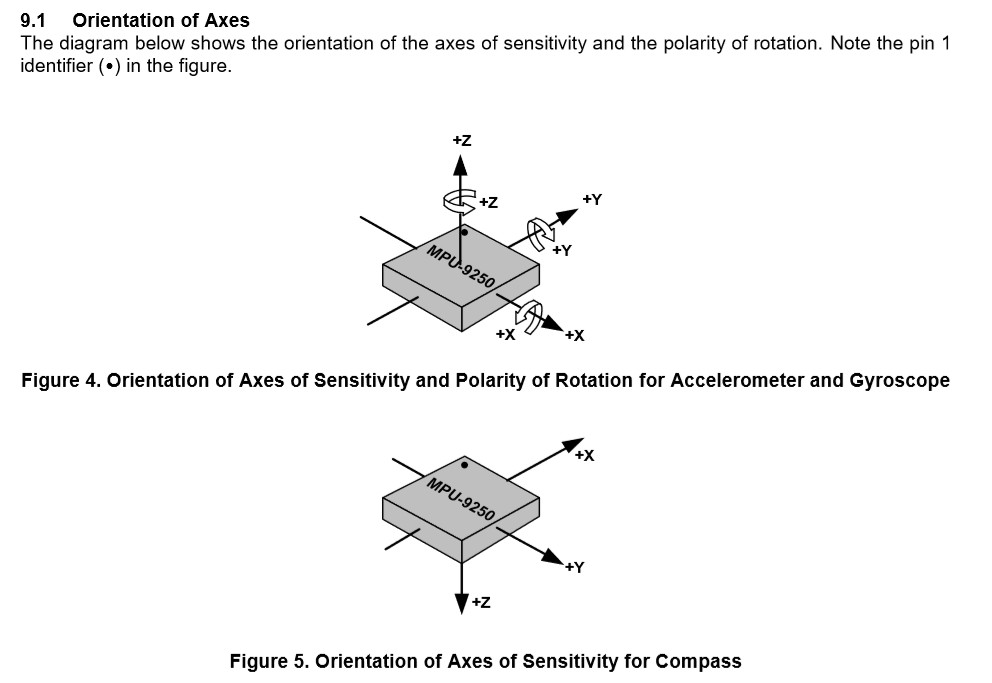
\includegraphics[width=0.75\textwidth]{images/MPU9250_axisOrientation}
	\label{MPUAxisOrientation}
	\caption{Orientation of axes for MPU9250 data (page 38 of datasheet).}
\end{figure}


\begin{figure}
	\centering
	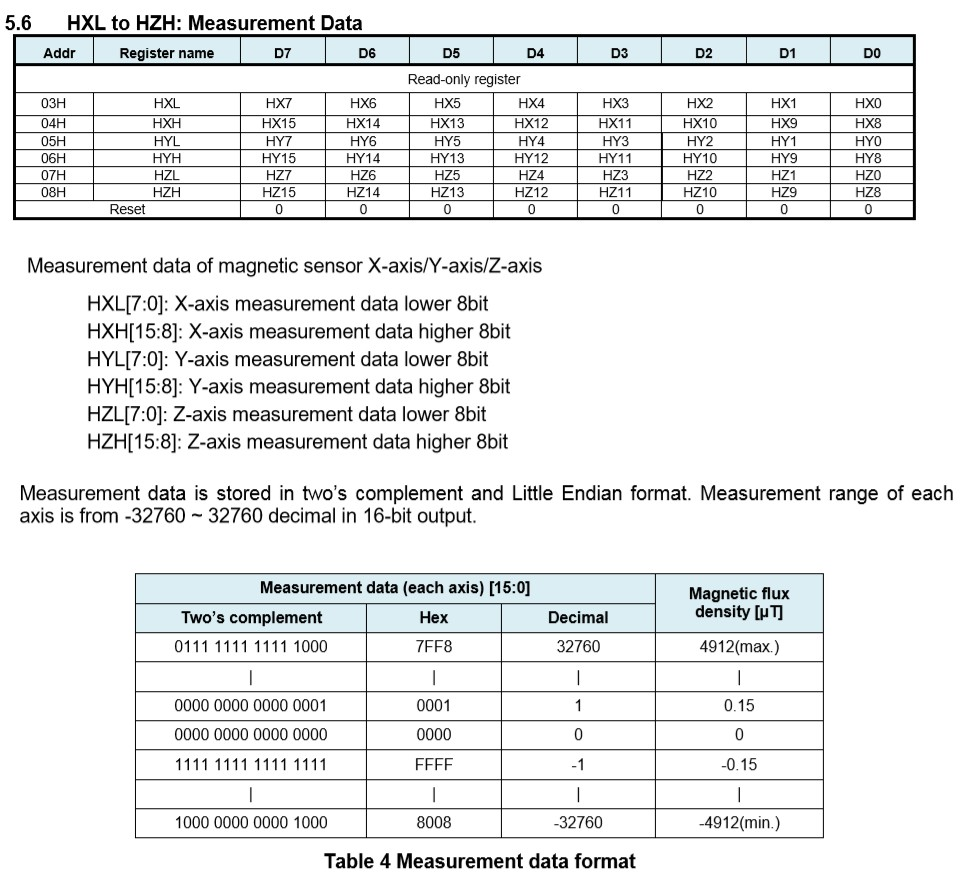
\includegraphics[width=0.75\textwidth]{images/MPU9250_magnetometerRegs}
	\label{MPUMagRegs}
	\caption{Magnetometer register map and corresponding scales from page 50 of the register map.}
\end{figure}

\clearpage

%
%
%
%

\section{18B20 (temperature sensor)} \label{tempsensor}
The temperature sensor is used to monitor the temperature of the electromagnet. It provides digital signal to the microcontroller for reading, strictly following a 1-wire protocol. Byte-long codes are listed in pages 10 through 12 of the datasheet, which are transmitted LSb first. Each sensor has a unique ROM address which can be identified using the Search ROM cycle documented on page 10 of the datasheet.
\clearpage

%
%
%
%

\section{DRV8871 (H-bridge)} \label{hbridge}
The H-bridges are used to generate magnetic fields of various strengths in the coils surrounding the fluid cell, and to generate various heat gradients using the TECs. PWM is used in both cases.
\clearpage

%
%
%
%

\section{TEC (thermoelectric cooler)} \label{18B20}
The TEC plates are used to supply heat and cooling to the fluid.

Power data should be acquired at about 500 Hz
\clearpage

%
%
%
%

\section{Integration} \label{integration}
The aforementioned components were integrated using a STM32F411RE microcontroller on a Nucleo-F411 development board.

\subsection{Data Logging}
Data from all sensors were logged and sent to the onboard PC over a 256 [kHz] UART channel. The packet format was as follows:

\begin{table}[!ht]
	\centering
	\begin{tabular}{ | m{3cm} | m{2cm} | m{2cm} | m{2cm}| m{2cm}| m{2cm}| m{2cm}|  } 
		\hline
		Parameter & Data Type & Size (bytes) & Offset (bytes) & Units & Range & Positive Sign Convention \\
		\hline
		Magnet power & TODO & TODO & TODO & TODO & TODO & TODO \\ 
		\hline
	    TEC power & TODO & TODO & TODO & TODO & TODO & TODO \\ 
		\hline
		Temperature & TODO & TODO & TODO & TODO & TODO & TODO \\ 
		\hline
		Acceleration & TODO & TODO & TODO & TODO & TODO & TODO \\ 
		\hline
	\end{tabular}
	\caption{Form of packet to PC}
	\label{tab:PCPacketFormat}
\end{table}

Additionally, the aircraft provided its own data as a UDP packet on port 5124, which could be read by the onboard PC so long as it had an IP address of 132.246.192.[25..50]. A breakdown of the packet can be found in ``NRC Nav Packet.xlsx".
\clearpage

% ----------------------------------------------------------------
\end{document}
